\documentclass[shownotes, xcolor = table]{beamer}

\usepackage{xeCJK}
% \usepackage{zhnumber}	% counters in Chinese
\usepackage{fontspec}
\usepackage{comment}
\usepackage{xifthen}
\usepackage{verbatim}
\usepackage{lmodern}

\usetheme{CambridgeUS} % try Madrid
\usecolortheme{beaver} % try beaver, dolphin, seahorse
\usefonttheme[onlymath]{serif} % try "professionalfonts"
% \setCJKmainfont{SimSun} % try SimSun

\usepackage{tikz}
\usetikzlibrary{chains, arrows.meta, shapes, positioning, calc, backgrounds, fit}

\usepackage{amsmath, amsfonts, amssymb, mathtools, pifont}
\newcommand{\cmark}{\ding{51}}%
\newcommand{\xmark}{\ding{55}}%
\def\checkmark{\tikz\fill[scale=0.5](0,.35) -- (.25,0) -- (1,.7) -- (.25,.15) -- cycle;} 

\usepackage{graphicx, subcaption}
\usepackage[export]{adjustbox}

\usepackage[framemethod=TikZ]{mdframed}

\usepackage[normalem]{ulem} % strike through text
\newcommand{\soutthick}[1]{%
    \renewcommand{\ULthickness}{2.0pt}%
       \sout{#1}%
    \renewcommand{\ULthickness}{.4pt}% Resetting to ulem default
}

\setbeamersize{text margin left = 2em, text margin right = 1em}
\setbeamercolor{footnote mark}{fg = teal}
\setbeamertemplate{itemize items}[default]
\setbeamertemplate{enumerate items}[default]

% for algorithms
\usepackage{algorithm}
\usepackage[noend]{algpseudocode} % also loading algorithmicx
\ExplSyntaxOn
\bool_new:N \l__xeCJK_listings_letter_bool % workaround
\ExplSyntaxOff
\usepackage{listings}
\usepackage{textcomp}

\newcommand{\hStatex}[0]{\vspace{5pt}}
\newcommand{\algvariable}[1]{\texttt{#1}}
\newcommand{\algkeyword}[1]{\textbf{#1}}
\newcommand{\algprocedure}[1]{\textsc{#1}}

% lComment: line comment; mComment: margin comment
\algnewcommand{\lComment}[1]{\State \emph{$\triangleright$ #1}}
\algnewcommand{\lendComment}[1]{\State \textcolor{violet}{\emph{$\triangleleft$ #1}}}
\algnewcommand{\mComment}[1]{\Comment{\emph{#1}}}

\algblockdefx{BeginRepeat}{EndRepeat}{\textbf{repeat}}{}
\algnotext{EndRepeat}

\newcommand{\attr}[1]{\textsl{#1}}
\newcommand{\msg}[2]{$\langle \textup{\scriptsize #1}, #2 \rangle$}

% for tables
\usepackage{multirow}
\newcommand{\innercell}[2]{\begin{tabular}{@{}#1@{}}#2\end{tabular}}
\usepackage{hhline}
%%%%%%%%%%%%%% for appendix %%%%%%%%%%%%%%%%
% http://www-ljk.imag.fr/membres/Jerome.Lelong/latex/appendixnumberbeamer.sty
% Reference: http://tex.stackexchange.com/questions/2541/beamer-frame-numbering-in-appendix
\usepackage{appendixnumberbeamer}
% Add total frame count to slides, optional. From Stefan,
% http://www.latex-community.org/forum/viewtopic.php?f=4&t=2173
\expandafter\def\expandafter\insertshorttitle\expandafter{%
  \insertshorttitle\hfill\insertframenumber\,/\,\inserttotalframenumber}
%%%%%%%%%%%%%% for appendix %%%%%%%%%%%%%%%%

% for fig without caption: #1: width/size; #2: fig file
\newcommand{\fignocaption}[2]{
  \begin{figure}[htp]
    \centering
    \includegraphics[#1]{#2}
  \end{figure}
}

% for fig with caption: #1: width/size; #2: fig file; #3: fig caption
\newcommand{\fig}[3]{
  \begin{figure}[htp]
    \centering
      \includegraphics[#1]{#2}
      \caption{#3}
  \end{figure}
}

% for cite: #1: author; #2: conference #3: year
\newcommand{\citeinbeamer}[3]{{\scriptsize{\textcolor{blue}{[#1@#2'#3]}}}}

\usepackage[backend=bibtex]{biblatex}
\addbibresource{phd-defense-report.bib}

\newcommand{\set}[1]{\{#1\}}
\newcommand{\question}[1]{\textcolor{red}{\centerline{#1}}}
\newcommand{\answer}[1]{\textcolor{blue}{\centerline {#1}}}
\newcommand{\alertred}[1]{\textcolor{red}{#1}}
\newcommand{\alertblue}[1]{\textcolor{blue}{#1}}
\newcommand{\todo}[1]{\textcolor{red}{\textbf{TODO:} #1}}
\newcommand{\mathbfblue}[1]{\textcolor{blue}{$\mathbf{#1}$}}

\newcommand{\papertitle}{Parameterized and Runtime-tunable Snapshot Isolation in Distributed Transactional Key-value Stores}
\newcommand{\shortpapertitle}{Parameterized and Runtime-tunable Snapshot Isolation}

\newcommand{\putop}{\texttt{put(K key, V val)}}
\newcommand{\getop}{\texttt{get(K key)}}

\newcommand{\red}[1]{\textcolor{red}{#1}}
\newcommand{\blue}[1]{\textcolor{blue}{#1}}

\newcommand{\timeprech}{\prec_{h}}
\newcommand{\timepreceqh}{\preceq_{h}}

\newcommand{\hp}{\prec_{h}}
\newcommand{\aca}{\text{ACA}}
\newcommand{\wcf}{\text{WCF}}
\newcommand{\rc}{\text{RC}}
\newcommand{\si}{\text{SI}}
\newcommand{\rvsi}{\text{RVSI}}
\newcommand{\konebv}{k_1\text{-BV}}
\newcommand{\ktwofv}{k_2\text{-FV}}
\newcommand{\kthreesv}{k_3\text{-SV}}
\newcommand{\chameleon}{\textsc{Chameleon}}

\newcommand{\algnamefont}[1]{#1}
\newcommand{\rvsims}{\algnamefont{RVSI-MS}}
\newcommand{\rvsimp}{\algnamefont{RVSI-MP}}
\newcommand{\ebegin}{\textsc{Begin}}
\newcommand{\eread}{\textsc{Read}}
\newcommand{\ewrite}{\textsc{Write}}
\newcommand{\eend}{\textsc{End}}
\newcommand{\estart}{\textsc{Start}}
\newcommand{\ecommit}{\textsc{Commit}}
\newcommand{\esend}{\textsc{Send}}
\newcommand{\ereceive}{\textsc{Receive}}

\newcommand{\master}{\mathcal{M}}
\newcommand{\slave}{\mathcal{S}}
\newcommand{\coordinator}{\mathcal{C}}
\newcommand{\timeoracle}{\mathcal{T}}
\newcommand{\tots}{$\timeoracle$.\attr{ts}}
\newcommand{\tvc}[1]{#1.\attr{vc}}
\newcommand{\tws}[1]{#1.\attr{writes}}
\newcommand{\tcts}[1]{#1.\attr{cts}}
\newcommand{\mpord}[1]{\mathcal{O}_{#1}}


\title[RVSI@SRDS, HongKong]{\papertitle}
% \subtitle{(SRDS 2017, HongKong)}

\author[Hengfeng Wei]{\textbf{Hengfeng Wei}, Yu Huang, Jian Lu}
\titlegraphic{
\includegraphics[height = 1.3cm]{figs/nju-logo-purple.png}~
\includegraphics[height = 1.3cm]{figs/cs-logo.jpg}}
% \institute{Institute of Computer Software \\ Nanjing University}
\institute{Nanjing University, China}
\date{\today}

\AtBeginSection[]{
  \begin{frame}[noframenumbering, plain]
    \frametitle{\shortpapertitle}
    \centerline{\underline{\large RVSI: Relaxed Version Snapshot Isolation}}
    \tableofcontents[currentsection, sectionstyle=show/shaded, subsectionstyle=hide/hide/hide]
  \end{frame}
}
%%%%%%%%%%%%%%%%%%%%
\begin{document}

% mdf: mdframed; #1: frame color; #2: frame title color; #3: frame title; #4: text
\newcommand{\mdf}[4]{
\begin{mdframed}[frametitle={
  \tikz[baseline = (current bounding box.east), outer sep = 0pt]
  \node[anchor = east, rectangle, fill = #1!20, font = \small]{\strut \textcolor{#2}{#3}};},
  innertopmargin = 2pt, linecolor = #1!20, linewidth = 2pt, topline = true,
  frametitleaboveskip=\dimexpr-\ht\strutbox\relax]
  #4
\end{mdframed}
}

\maketitle

\begin{frame}[noframenumbering, plain]
  \frametitle{\shortpapertitle}
  \centerline{\underline{\large RVSI: Relaxed Version Snapshot Isolation}}
  \tableofcontents[currentsection, sectionstyle=show, subsectionstyle=show/show/hide]
\end{frame}

\section{Motivation for RVSI}

%%%%%%%%%%%%%%%
\begin{frame}{}
  \centerline{Distributed key-value stores:}
  \fignocaption{width = 0.50\textwidth}{figs/kvs.pdf}
  \centerline{\putop{} \qquad \getop{}}
\end{frame}
%%%%%%%%%%%%%%%

%%%%%%%%%%%%%%%
\begin{frame}{}
  \begin{center}
    Transactions are performed on \red{a group of keys} in an ``all-or-none'' way.
  \end{center}

  \pause
  \vspace{0.50cm}
  \fignocaption{width = 0.55\textwidth}{figs/consistency-model-tree.png}
  \centerline{Transactional consistency models (from \citeinbeamer{Bailis}{VLDB}{14})}
\end{frame}
%%%%%%%%%%%%%%%

%%%%%%%%%%%%%%%
\begin{frame}{}
  Snapshot isolation (SI \citeinbeamer{Berenson}{SIGMOD}{95}, \citeinbeamer{Adya}{Thesis}{99}):
  \begin{itemize}
    \item Each transaction \red{reads} from the ``latest'' snapshot as of the time it started.
    \item If multiple concurrent transactions \red{write} to the same data item,
      at most one of them will commit. \hfill (WCF: \emph{write-conflict freedom})
  \end{itemize}
\end{frame}
%%%%%%%%%%%%%%%

%%%%%%%%%%%%%%%
\begin{frame}{}
  \begin{center}
    Reading the \red{``latest''} in a \blue{distributed} setting \\
    often requires intensive coordinations.
  \end{center}

  \pause
  \vspace{0.50cm}
  Relaxed variants of (distributed) SI:
  \begin{description}[PL-FCVpad]
    \item[GSI~\footnote{GSI: Generalized Snapshot Isolation \citeinbeamer{Elnikety}{SRDS}{05}}:]
      allows to read from ``older'' snapshots
    \item[NMSI~\footnote{NMSI: Non-Monotonic Snapshot Isolation \citeinbeamer{Ardekani}{SRDS}{13}}:]
      allows to observe non-monotonically ordered snapshots
    \item[PL-FCV~\footnote{PL-FCV: Forward Consistent View \citeinbeamer{Aday}{Thesis}{99}}:]
      allows a transaction to observe the updates of transactions that commit after it started
    \item[PSI~\footnote{PSI: Parallel Snapshot Isolation \citeinbeamer{Sovran}{SOSP}{11}}:]
      causal ordering of transactions across sites
  \end{description}
\end{frame}
%%%%%%%%%%%%%%%

%%%%%%%%%%%%%%%
\begin{frame}{}
  Two possible drawbacks:
  \begin{enumerate}
    \setlength{\itemsep}{8pt}
    \item Unbounded inconsistency
      \begin{itemize}
	\item no specification of the severity of the anomalies w.r.t SI
      \end{itemize}
    \pause
    \item Untunable at runtime
      \begin{itemize}
	\setlength{\itemsep}{5pt}
	\item determined at the system design phase
	\item remain unchanged once the system is deployed
      \end{itemize}
  \end{enumerate}
\end{frame}
%%%%%%%%%%%%%%%

%%%%%%%%%%%%%%%
\begin{frame}{}
  \begin{center}
    An online bookstore application~\footnote{Adapted from \citeinbeamer{Guo}{SIGMOD}{04} 
    and \citeinbeamer{Bernstein}{SIGMOD}{06}.} for motivating \\
    \red{\large ``bounded inconsistency''} and \red{\large ``runtime-tuable''}:
  \end{center}

  \vspace{-0.20cm}
  \begin{table}
    \centering
    \begin{tabular}{c|c|c|c|c|c|c}
      \hline
      Title & Authors & Sales & Inventory & Ratings & Reviews & $\cdots$ \\
      \hline
    \end{tabular}
  \end{table}

  \pause
  \vspace{0.20cm}
  \begin{description}[Bookstore Clerk ($T_2$):]
    \setlength{\itemsep}{6pt}
    \item[Customer ($T_1$):] Obtaining the basic info. about a book
      \begin{itemize}
	\item \emph{\blue{out-of-date}} reviews
      \end{itemize}
      \pause
    \item[Bookstore Clerk ($T_2$):] Checking the inventory of a book
      \begin{itemize}
	\item inventory updated by concurrent transactions committed \emph{\blue{after}} $T_2$ starts
      \end{itemize}
      \pause
    \item[Sales Analyst ($T_3$):] Studying sales vs. ratings of a book
      \begin{itemize}
	\item sales and ratings from \emph{\blue{separate snapshots}}
      \end{itemize}
  \end{description}
\end{frame}
%%%%%%%%%%%%%%%

%%%%%%%%%%%%%%%
\begin{frame}{}
  The idea of {\large ``\red{parameterized} and \blue{runtime-tunable} snapshot isolation''}.

  \vspace{0.50cm}
  \red{\rvsi{}}: Relaxed Version Snapshot Isolation
  \begin{description}
    \item[$\konebv$:] $k_1$-version bounded \emph{\red{backward}} view
    \item[$\ktwofv$:] $k_2$-version bounded \emph{\red{forward}} view
    \item[$\kthreesv$:] $k_3$-version bounded \emph{\red{snapshot}} view
  \end{description}

  \pause
  \vspace{10pt}
  \blue{\chameleon{}}: a prototype distributed transactional key-value store
  \begin{itemize}
    \item Achieves \rvsi{}
    \item Allows each transaction to tune its consistency level at runtime
      \pause
    \item Deployed on Aliyun~\footnote{\url{http://www.aliyun.com/}}
    \item Evaluates the impacts of \rvsi{} on the transaction abort rates
  \end{itemize}
\end{frame}
%%%%%%%%%%%%%%%

\section{Definition of RVSI}

% % si
%%%%%%%%%%%%%%%
\begin{frame}{}
    Transaction $T_i$:
    \begin{itemize}
      \item begins with a \texttt{start} operation $s_i$ 
      \item contains a sequence of \texttt{read} or \texttt{write} operations
      \item ends with a \texttt{commit} operation $c_i$ or an \texttt{abort} operation $a_i$
    \end{itemize}

    \pause
    \vspace{0.30cm}
    History: modelling an execution of a transactional key-value store
    \begin{itemize}
      \item $w_i(x_i)$: transaction $T_i$ writing version $i$ of data item $x$
      \item $r_i(x_j)$: transaction $T_i$ reading version $j$ of data item $x$ written by $T_j$
      \item \emph{time-precedes partial order} $\timeprech$ over operations
      \item $T_i$ and $T_j$ are concurrent:
	\[
	  s_i \timeprech c_j \land s_j \timeprech c_i
	\]
    \end{itemize}
\end{frame}
%%%%%%%%%%%%%%%

%%%%%%%%%%%%%%%
\begin{frame}{}
  Snapshot isolation requires that:
  \begin{description}[Snapshot Write:]
    \item[Snapshot Read:] Each transaction read data from the ``lastest'' snapshot as of the time the transaction started.
    \item[Snapshot Write:] No \red{write}-conflicting concurrent transactions
  \end{description}
\end{frame}
%%%%%%%%%%%%%%%

%%%%%%%%%%%%%%%
\begin{frame}{}
  A history $h$ is in snapshot isolation if and only if it satisfies \citeinbeamer{Adya}{Thesis}{99} \\[0.20cm]
  \begin{description}[Snapshot Write:]
    \item[Snapshot Read:] All reads of transaction $T_i$ occur at $T_i$'s start time.
      \begin{align*}
	\forall &r_i(x_{j \neq i}), w_{k \neq j}(x_k), c_k \in h: \\
	& (c_j \in h \land c_j \timeprech s_i)
	 \land (s_i \timeprech c_k \lor c_k \timeprech c_j).
      \end{align*}
    \item[Snapshot Write:] No concurrent committed transactions may write the same data item.
      \begin{align*}
	\forall w_i(x_i), w_{j \neq i}(x_j) \in h \implies (c_i \timeprech s_j \lor c_j \timeprech s_i).
      \end{align*}
  \end{description}
\end{frame}
%%%%%%%%%%%%%%%

%%%%%%%%%%%%%%%
\begin{frame}{}
\end{frame}
%%%%%%%%%%%%%%%

%%%%%%%%%%%%%%%
\begin{frame}{}
\end{frame}
%%%%%%%%%%%%%%%

%%%%%%%%%%%%%%%
\begin{frame}{}
\end{frame}
%%%%%%%%%%%%%%%

%%%%%%%%%%%%%%%
\begin{frame}{}
\end{frame}
%%%%%%%%%%%%%%%

%%%%%%%%%%%%%%%
\begin{frame}{}
\end{frame}
%%%%%%%%%%%%%%%


%%%%%%%%%%%%%%%
\begin{frame}{Principle of \rvsi{}}
  \begin{itemize}
    \setlength{\itemsep}{10pt}
    \item<1-> Parameters ($k_1, k_2, k_3$) to control the severity of the anomalies w.r.t SI
    \item<2-> $\rc{}~\footnotemark \supset \rvsi(k_1, k_2, k_3) \supset \si{}$
    \item<2-> $\rvsi(\infty,\infty,\infty) = \rc \qquad \rvsi(1,0,\ast) = \si$
  \end{itemize}
  \footnotetext{RC: Read Committed}
\end{frame}
%%%%%%%%%%%%%%%

%%%%%%%%%%%%%%%
\begin{frame}{Principle of \rvsi{}}
  \begin{quote}
    $\ldots$\\
    \hfill -- ``Snapshot Read'' property of SI
  \end{quote}

  \begin{enumerate}[<+->]
    \setlength{\itemsep}{10pt}
    \item ``stale'' data versions		\hfill \uncover<4->{\red{bounded staleness}}
    \item ``concurrent'' data versions  	\hfill \uncover<5->{\red{bounded concurrency level}}
    \item ``non-snapshot'' data versions	\hfill \uncover<6->{\red{bounded distance}}
  \end{enumerate}
\end{frame}
%%%%%%%%%%%%%%%

%%%%%%%%%%%%%%%
\begin{frame}{Illustration of RVSI}
  \fignocaption{width = 0.85\textwidth}{figs/rvsi-definition.pdf}
\end{frame}
%%%%%%%%%%%%%%%

%%%%%%%%%%%%%%%
\begin{frame}{Definition of RVSI}
  \begin{align*}
    & \red{(\konebv{})} \\
    \forall r_i(x_{j}), w_k(x_k), c_k \in h: 
    & \left(c_j \in h \land \bigwedge_{k=1}^{m} \left(c_j \hp c_k \hp s_i \right)\right) \Rightarrow m < k_1, \\[10pt]
    & \red{(\ktwofv{})} \\
    \forall r_i(x_{j}), w_k(x_k), c_k \in h:
    & \left(c_j \in h \land \bigwedge_{k=1}^{m} \left(s_i \hp c_k \hp c_j \right)\right) \Rightarrow m \le k_2, \\[10pt]
    & \red{(\kthreesv{})} \\
    \forall r_i(x_j), r_i(y_l), w_k(x_k), c_k \in h:
    & \left(\bigwedge_{k=1}^{m} \left(c_j \hp c_k \hp c_l \right)\right) \Rightarrow m \le k_3.
  \end{align*}
\end{frame}
%%%%%%%%%%%%%%%

%%%%%%%%%%%%%%%
\begin{frame}{Definition of \rvsi{}}
  \begin{equation*}
    h \in \rvsi{} \iff h \in \konebv{} \cap \ktwofv{} \cap \kthreesv{} \cap \wcf{}.
  \end{equation*}

  \vspace{0.50cm}
  \begin{theorem}
    \[
      \emph{\rvsi}(1,0,\ast) = \emph{\si}.
    \]
  \end{theorem}
\end{frame}
%%%%%%%%%%%%%%%

%%%%%%%%%%%%%%%
\begin{frame}{}
\end{frame}
%%%%%%%%%%%%%%%

%%%%%%%%%%%%%%%
\begin{frame}{}
\end{frame}
%%%%%%%%%%%%%%%

\section{\chameleon{} Prototype and RVSI Protocol}

% System Design of \chameleon{}

%%%%%%%%%%%%%%%
\begin{frame}{}
  \begin{center}
    \chameleon{} prototype: \\[10pt]
    A prototype \textbf{partitioned} \textbf{replicated} \\[6pt]
    distributed transactional \textbf{key-value} store
  \end{center}
\end{frame}
%%%%%%%%%%%%%%%

%%%%%%%%%%%%%%%
\begin{frame}{}
  \begin{center}
    Classic \textbf{key-value} data model \\[4pt]
      Key: (row key, column key)
  \end{center}
\end{frame}
%%%%%%%%%%%%%%%

%%%%%%%%%%%%%%%
\begin{frame}{}
  % \fignocaption{width = 0.70\textwidth}{figs/chameleon-arch.pdf}
  \begin{center}
    \resizebox{0.70\textwidth}{!}{%        File: chameleon-arch.tex
%     Created: Mon Jan 04 08:00 PM 2016 C
% Last Change: Mon Jan 04 08:00 PM 2016 C
% 	    Used in Beamer

\begin{tikzpicture}[connection/.style = {>=Stealth, <->, brown, dashed, line width = 3pt}]
  % background: china map
  \node (china-map) [opacity = 0.20] {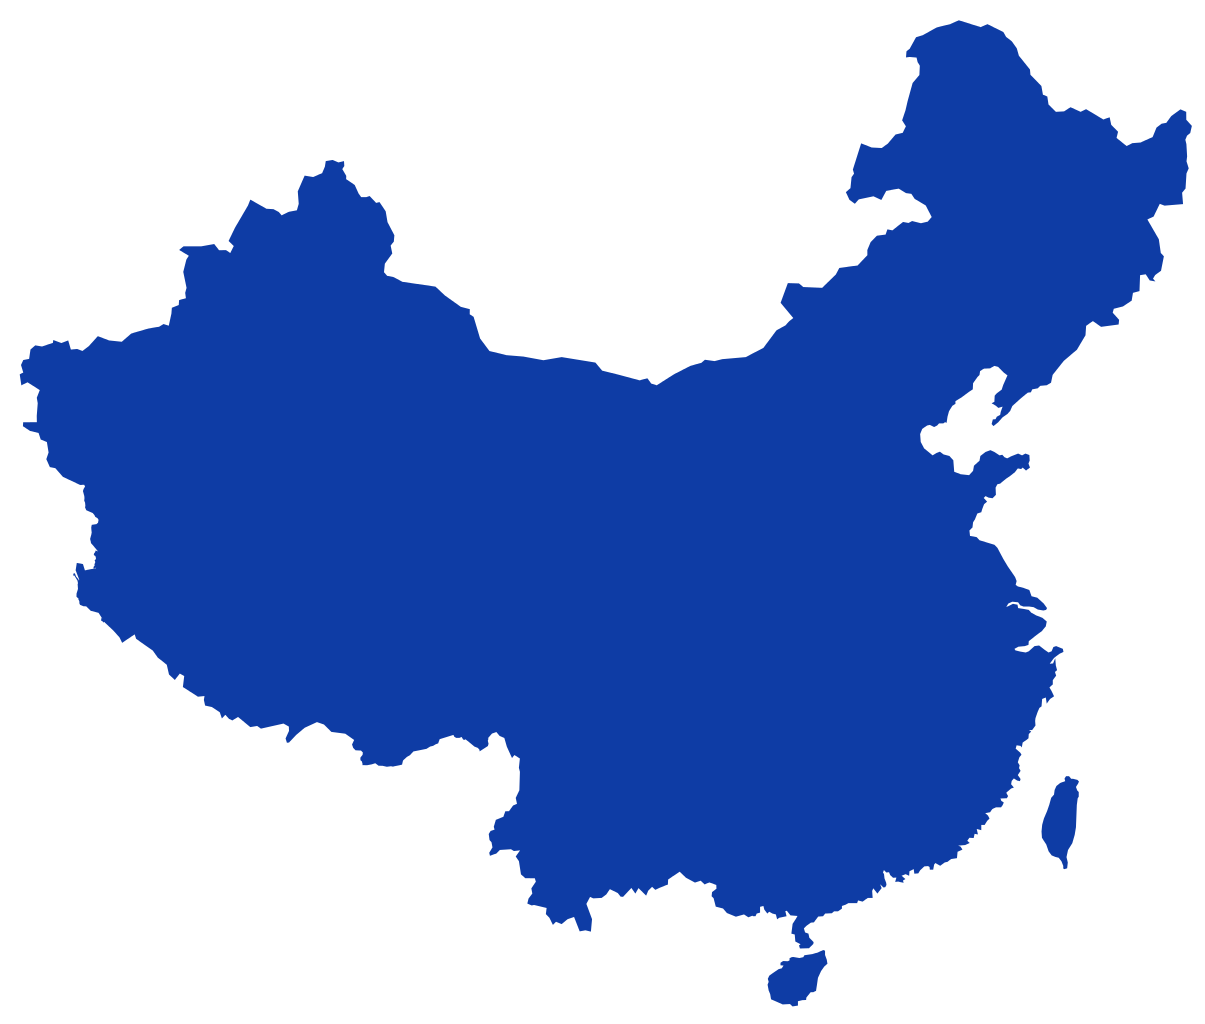
\includegraphics[scale = 0.40]{figs/china-outline-blue.png}};

  % partition-left, partition-right, partition-below
  \uncover<2->{
    \node (partition-left) [] at (-6.5, 1) {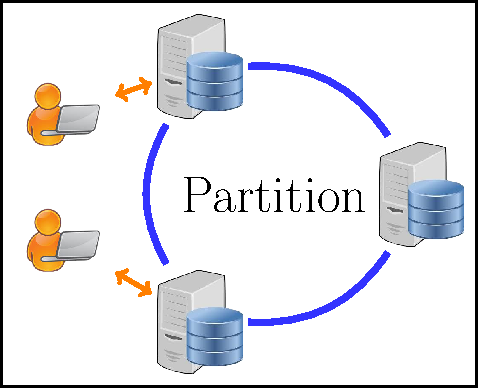
\includegraphics[scale = 0.80]{figs/partition.pdf}}; 
  }
  \uncover<3->{
    \node (partition-right) [] at (6, 3.5) {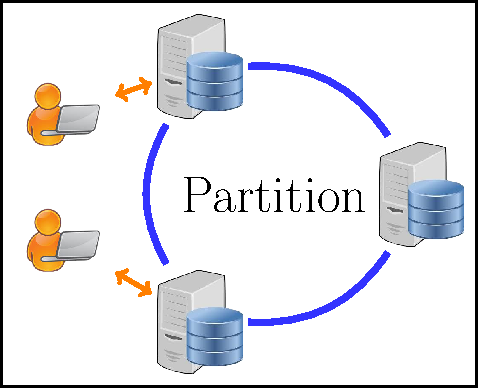
\includegraphics[scale = 0.80]{figs/partition.pdf}}; 
    \node (partition-below) [] at (1.5, -5) {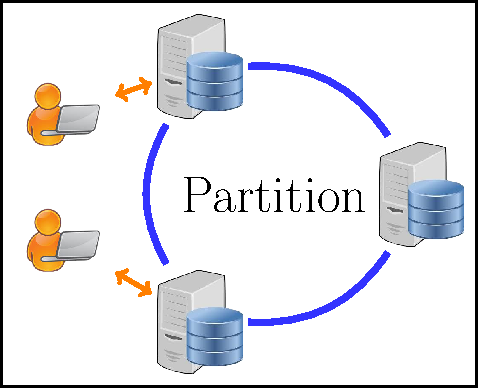
\includegraphics[scale = 0.80]{figs/partition.pdf}}; 

    % connections among partitions
    \draw [connection] (partition-left) to (partition-right); 
    \draw [connection] (partition-right) to (partition-below);
    \draw [connection] (partition-below) to (partition-left);

    % replication 
    \node (replication) [font = \Huge, align = center] at (0.5, 0.0) {\textbf{Wide-area}\\[3pt]\textbf{Replication}};
  }

  \uncover<4->{
    % master-slave for one partition
    \begin{scope}[circled/.style = {draw, circle, dash pattern = on 10pt off 5pt, cyan, line width = 2pt, outer sep = 5pt, minimum size = 2.0cm}, 
      conn/.style = {dash pattern = on 15pt off 8pt, cyan, line width = 2pt}]
    \node (ms-left) [circled] at (-4., 1) {};
    \node (ms-right) [circled] at (5.5, 1.7) {};
    \node (ms-below) [circled] at (4., -5.0) {};

    \node (master-slave) [below right = 1.5cm and -1.5cm of partition-right] {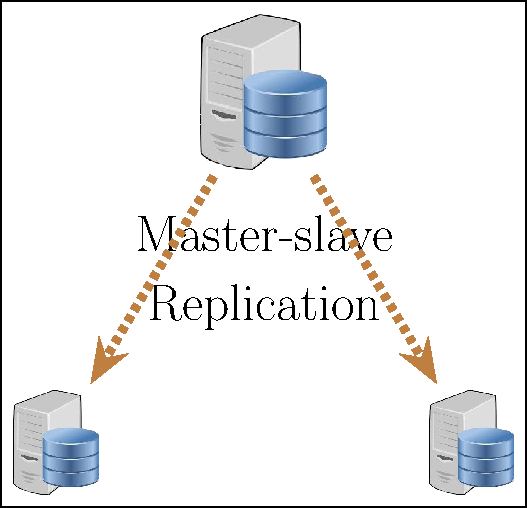
\includegraphics[scale = 0.80]{figs/master-slave.pdf}};
    \draw [conn] (ms-left) to (master-slave);
    \draw [conn] (ms-right) to (master-slave);
    \draw [conn] (ms-below) to (master-slave);
    \end{scope}
  }
\end{tikzpicture}
}
  \end{center}

  \begin{center}
    \only<2>{Keys are \textbf{partitioned} within a single datacenter.}
    \only<3-4>{Each key is \textbf{replicated} across datacenters} \only<4>{in a \textbf{master-slave} manner.}
    \only<5>{Transactions are first executed and committed on the \textbf{masters},\\
      and are then asynchronously propagated to \textbf{slaves}.}
  \end{center}
\end{frame}
%%%%%%%%%%%%%%%

%%%%%%%%%%%%%%%
\begin{frame}{}
  \only<1-3, 5->{\fignocaption{width = 0.50\textwidth}{figs/chameleon-framework.pdf}}

  \begin{center}
    \only<2>{\blue{1.} Partitioned replicated transactional key-value store}
    \only<3>{\blue{2.} Client library}
    \only<5>{\blue{3.} \rvsi{} protocol: \rvsims{} + \rvsimp{}}
  \end{center}

  \only<4>{
    Code snippet for writing \rvsi{} transactions: \\[8pt]
    \begin{lstlisting}[
  language = Java,
  basicstyle = \ttfamily\footnotesize,
  showstringspaces = false,
  keywordstyle = \color{blue}\bfseries,
  commentstyle = \color{teal},
  stringstyle = \bfseries,
  upquote = true,
  frame = box,
  breaklines = true,
  linewidth = 0.85\textwidth
]
  // Initialize keys (ck, ck1, and ck2) here
  ITx tx = new RVSITx(/** context **/);

  tx.begin();

  // Read and write
  ITsCell tsCell = tx.read(ck);
  ITsCell tsCell1 = tx.read(ck1);
  tx.write(ck1, new Cell("R1C1"));
  ITsCell tsCell2 = tx.read(ck2);

  // Specify RVSI specs. (e.g., SVSpec)
  RVSISpec sv = new SVSpec();
  sv.addSpec({ck, ck1, ck2}, 2);
  tx.collectRVSISpec(sv);

  boolean committed = tx.end();
\end{lstlisting}

  }
\end{frame}
%%%%%%%%%%%%%%%


% the RVSI-MS protocol
%%%%%%%%%%%%%%%
\begin{frame}{}
  \centerline{\rvsims{}: RVSI protocol for Master-Slave replication}

  \vspace{-0.80cm}
  \begin{center}
    \resizebox{0.50\textwidth}{!}{\begin{tikzpicture}[
  msg/.style = {>=Stealth, <->, very thick}]
  \node (ms) [] {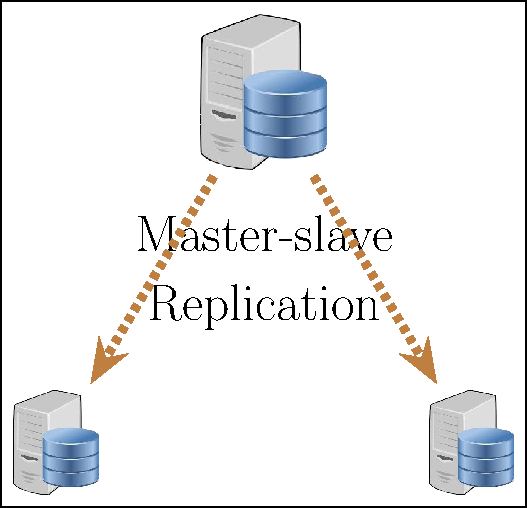
\includegraphics[scale = 0.40]{figs/master-slave.pdf}};
  \node (client) [above = 2.0cm of ms] {
\includegraphics[scale = 0.25]{figs/client-pc-logo.png}};

  \uncover<2->{
    % begin
    \draw [msg] (client) to node () [below = 5pt, midway, sloped] {\textsc{Begin}} 
    node () [above = 5pt, midway, sloped] {$T$.sts} (ms);
  }

  \uncover<3->{
    % read
    \draw [msg] (client) to [bend right = 40] node () [above = 5pt, midway, sloped] {\textsc{Read}} 
    ($(ms.south west) + (0,20pt)$);
  }

  \uncover<4->{
    % write
    \draw [msg] (client) to [out = -30, in = 30, looseness = 5] node () [] {\textsc{Write}} (client);
  }

  \uncover<5->{
    % commit
    \draw [msg] (client) to [bend left = 60] node () [below = 5pt, midway, sloped] {\textsc{Commit}} 
    node () [above = 5pt, midway, sloped] {$T$.cts} ($(ms.north) + (25pt, 0)$);
  }

  \uncover<6->{
    % vc
    \node () [below right = 0.10cm and 0.20cm of client.south, red] {$\textsc{ADD-VC}$};
    \node () [below right = 0.50cm and 0.20cm of ms.north, red] {\textsc{CHECK-VC}};
  }
\end{tikzpicture}}
  \end{center}

%   \vspace{1.0cm}
%   In terms of \emph{event} generation and handling:
%   \begin{description}
%     \item[Clients:] \ebegin, \eread, \ewrite, \eend%
%     \item[Master:] \estart, \ecommit, \esend%
%     \item[Slaves:] \ereceive%
%   \end{description}
\end{frame}
%%%%%%%%%%%%%%%

%%%%%%%%%%%%%%%
\begin{frame}{}
  Calculating version constraints for \rvsi{}: 

  \[
    \mathcal{O}_{x}(t) = \text{\# of versions of } x \text{ before time } t % \max \set{x.\attr{ord} \mid x.\attr{ts} \le t}
  \]

  \[
    \blue{r_i(x_j) \in T_i}
  \]
  \vspace{-0.40cm}
  \begin{description}
    \item[$\konebv$:]
      \[
	\mathcal{O}_{x}(T_i.\textsl{sts}) - \mathcal{O}_{x}(T_j.\textsl{cts}) < k_1
      \]
    \item[$\ktwofv$:]
      \[
	\mathcal{O}_{x}(T_j.\textsl{cts}) - \mathcal{O}_{x}(T_i.\textsl{sts}) \le k_2
      \]
    \pause
    \item[$\kthreesv$:]
      \[
	\blue{r_i(x_j), r_i(y_l) \in T_i}
      \]
      \vspace{-0.40cm}
      \[
	\mathcal{O}_{\red{x}}(T_l.\textsl{cts}) - \mathcal{O}_{\red{x}}(T_j.\textsl{cts}) \le k_3
      \]
  \end{description}
\end{frame}
%%%%%%%%%%%%%%%

% the RVSI-MP protocol
%%%%%%%%%%%%%%%
\begin{frame}{}
  \begin{center}
    \rvsimp{}: \rvsi{} protocol for Multiple Partitions\\[10pt]
    Distributed transactions spanning multiple masters \\
    need to be committed atomically.

    \pause
    \vspace{0.40cm}
    Using the two-phase commit (2PC) protocol \citeinbeamer{Bernstein}{Book}{87}.

    \pause
    \vspace{1.00cm}
    We have two issues to address.
  \end{center}
\end{frame}
%%%%%%%%%%%%%%%

%%%%%%%%%%%%%%%
\begin{frame}{}
  Assumes a timestamp oracle \citeinbeamer{Peng}{OSDI}{10}:
  \begin{description}[Coordinator:]
    \item[Client:] asks for the start-timestamp in \textsc{Begin}
    \item[Coordinator:] asks for the commit-timestamp in \textsc{Commit}
  \end{description}
\end{frame}
%%%%%%%%%%%%%%%

%%%%%%%%%%%%%%%
\begin{frame}{}
  Split the \rvsi{} version constraints according to partitions:

  \[
    \blue{r_i(x_j) \in T_i}
  \]
  \vspace{-0.40cm}
  \begin{description}
    \item[$\konebv$:]
      \[
	\mathcal{O}_{\red{x}}(T_i.\textsl{sts}) - \mathcal{O}_{\red{x}}(T_j.\textsl{cts}) < k_1
      \]
    \item[$\ktwofv$:]
      \[
	\mathcal{O}_{\red{x}}(T_j.\textsl{cts}) - \mathcal{O}_{\red{x}}(T_i.\textsl{sts}) \le k_2
      \]
    \item[$\kthreesv$:]
      \[
	\blue{r_i(x_j), r_i(y_l) \in T_i}
      \]
      \vspace{-0.40cm}
      \[
	\mathcal{O}_{\red{x}}(T_l.\textsl{cts}) - \mathcal{O}_{\red{x}}(T_j.\textsl{cts}) \le k_3
      \]
  \end{description}

  \vspace{0.6cm}
  \centerline{All version constraints involve only one data item.}
\end{frame}
%%%%%%%%%%%%%%%

\section{Experimental Evaluation}

%%%%%%%%%%%%%%%
\begin{frame}{}
  \begin{center}
    Impacts of \rvsi{} specification \\[5pt]
    on the \emph{\blue{transaction abort rates}} in various scenarios
  \end{center}

  \pause
  \vspace{0.50cm}
  \centerline{\red{What about performance?}}
  \begin{itemize}
    \item Not done yet in this work
    \item \rvsims{} and \rvsimp{} protocols in \chameleon{} are simple
  \end{itemize}
\end{frame}
%%%%%%%%%%%%%%%

%%%%%%%%%%%%%%%
\begin{frame}{}
  \begin{columns}
    \column{0.50\textwidth}
      \chameleon{} prototype on Aliyun:
      \begin{itemize}
	\item 3 datacenters~\footnotemark[1]
	\item 3 nodes in each datacenter
	\item Partition \& Replication
	\item Clients in our lab~\footnotemark[2]
      \end{itemize}

      \vspace{0.60cm}
      \uncover<2->{
	(One-way) delays among nodes~\footnotemark[3]:
	\begin{description}[Across datacenters:]
	  \item[Within datacenter:] $1 \sim 2$ms
	  \item[Across datacenters:] $15 \sim 25$ms
	  \item[Clients to nodes:] $15 \sim 20$ms
	\end{description}
      }
    \column{0.50\textwidth}
      \fignocaption{width = 0.85\textwidth}{figs/chameleon-arch.pdf}
  \end{columns}

  \footnotetext[1]{Located in East China, North China, and South China, respectively.}
  \footnotetext[2]{Located in East China.}
  \footnotetext[3]{\url{https://github.com/hengxin/aliyun-ping-traces}}
\end{frame}
%%%%%%%%%%%%%%%

%%%%%%%%%%%%%%%
\begin{frame}{}
  \centerline{Three categories of workload parameters for experiments on Aliyun.}
  \begin{table}[!t]
  \centering
  \renewcommand*{\arraystretch}{1.2}
  \caption{Three categories of workload parameters for experiments on Aliyun.}
  % \resizebox{0.95\textwidth}{!}{%
    { %
  \begin{tabular}{|c|c||c|c|}
	\hline
    \multicolumn{2}{|c||}{\textbf{Parameter}} & \textbf{Value}		& \textbf{Explanation}
	\\ \hline  \hline
    \multirow{6}{*}{\bf Transaction-related}
    &\#keys  						& 25 = 5 (rows) $\times$ 5 (columns)  	&  	size of keyspace
	\\ \cline{2-4}
	&\#clients						& 5, 10, 15, 20, 25, 30 & number of clients
    \\ \cline{2-4}
	&\#txs/client					& 1000 & number of transactions per client
	\\ \cline{2-4}
	&\#ops/tx				& $\sim$ Binomial(20, 0.5) &  number of operations per transaction
	\\ \cline{2-4}
	&rwRatio							& 1:2, 1:1, 4:1 & {\#reads}/{\#writes}
	\\ \cline{2-4}
	&zipfExponent					& 1		& parameter for Zipfian distribution
	\\ \hline  \hline
    \multirow{3}{*}{\bf Execution-related} & minInterval						& 0ms		& minimum inter-transaction time
	\\ \cline{2-4}
	&maxInterval						& 10ms		& maximum inter-transaction time
	\\ \cline{2-4}
	&meanInterval					& 5ms		& mean inter-transaction time
    \\ \hline \hline
    {\bf RVSI-related} & $(k_1, k_2, k_3)$		
		&  \innercell{c}{(1,0,0) (1,1,0) (1,1,1) \\ (2,0,0) (2,0,1) (2,1,1)}	
		&  for $\konebv{}$, $\ktwofv{}$, and $\kthreesv{}$
	\\ \hline
  \end{tabular}}
  % }
\end{table}

\end{frame}
%%%%%%%%%%%%%%%

%%%%%%%%%%%%%%%
\begin{frame}{}
  Transactions abort for two reasons:
  \begin{itemize}
    \item \red{``vc-aborted''}: \rvsi{} version constraints violated
    \item \blue{``wcf-aborted''}: the WCF property violated
  \end{itemize}

  \pause
  \vspace{0.60cm}
  Transaction abort rates due to \red{``vc-aborted''} are \emph{sensitive} to different values of $k_1$, $k_2$, or $k_3$,
  \pause
  but those due to \blue{``wcf-aborted''} are not.

  \pause
  \vspace{0.50cm}
  \[
    h \in \rvsi{} \iff h \in \red{\konebv{}} \cap \red{\ktwofv{}} \cap \red{\kthreesv{}} \cap \blue{\wcf{}}.
  \]

  \pause
  \vspace{0.80cm}
  \centerline{\red{We report the results 
    under the read-frequent workloads~\footnote{\url{https://github.com/hengxin/chameleon-transactional-kvstore}}.}}
\end{frame}
%%%%%%%%%%%%%%%

%%%%%%%%%%%%%%%
\begin{frame}{}
  \fignocaption{width = 0.80\textwidth}{figs/aliyun-vc-rf.pdf}

  \pause
  The transaction abort rates due to ``vc-aborted'' \pause can be \red{greatly reduced}
  by \blue{slightly} increasing the values of $k_1$, $k_2$, or $k_3$:
  \[
    vc(1,0,0) = 0.1994 \implies vc(2,1,1) = 0.0091 \quad (\text{\#clients} = 30)
  \]
\end{frame}
%%%%%%%%%%%%%%%

%%%%%%%%%%%%%%%
\begin{frame}{}
  \fignocaption{width = 0.55\textwidth}{figs/aliyun-bvfvsv.pdf}

  \pause
  Most ``vc-aborted'' transactions abort because of violating \red{$\ktwofv$}.
  \[
    fv(1,0,0) = 0.1889 \implies fv(\blue{2},0,0) = 0.1866 \implies fv(1,\red{\bf 1},0) = 0.0064
  \]
\end{frame}
%%%%%%%%%%%%%%%

%%%%%%%%%%%%%%%
\begin{frame}{}
  \begin{center}
    \red{Question: when does $k_1$ for $\konebv$ take effect?} \\[10pt]
    It seems that $\konebv$ has \emph{\red{little}} impact on the transaction abort rates. \\[30pt]
    \pause
    It may be the case in the Aliyun scenarios. \\[10pt]
    \blue{What about other scenarios?}
  \end{center}
\end{frame}
%%%%%%%%%%%%%%%

%%%%%%%%%%%%%%%
\begin{frame}{}
  \centerline{Three types of delays for \blue{\large controlled experiments} on local hosts.}
  \begin{center}
    \begin{tikzpicture}[
  delay/.style = {>=Stealth, ->, very thick}]
  \node (client) [] {
\includegraphics[scale = 0.15]{figs/client-pc-logo.png}};
  \node (lms) [below left = 1.8cm and -0.5cm of client] {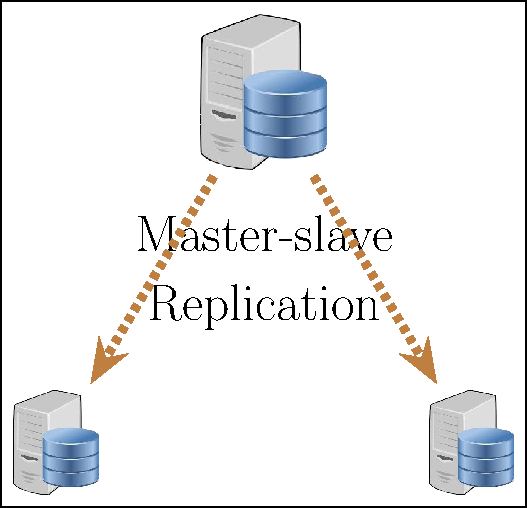
\includegraphics[scale = 0.30]{figs/master-slave.pdf}};
  \node (rms) [below right = 1.8cm and -0.5cm of client] {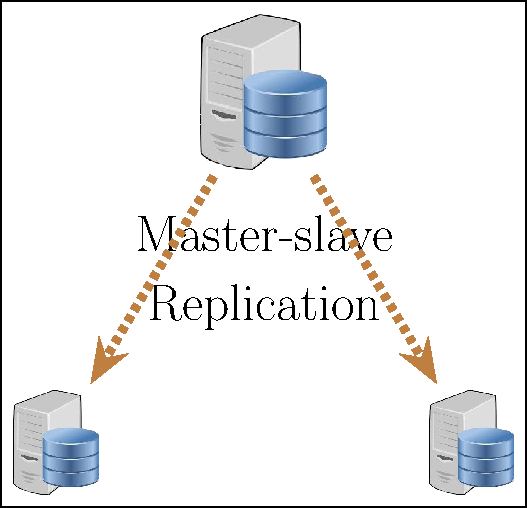
\includegraphics[scale = 0.30]{figs/master-slave.pdf}};

  \uncover<2->{
    % issue delay
    \draw [delay, cyan] (client) to node () [right = -8pt] {issueDelay} ($(lms.north) - (0, 2pt)$);
    \draw [delay, cyan] (client) to ($(rms.south west) + (10pt, 25pt)$);
  }

  \uncover<3->{
    % replication delay
    \draw [delay, teal] ($(rms.north) - (-15pt, 20pt)$) to [bend left] 
    node () [above, sloped] {replDelay} ($(rms.south east) - (15pt, -25pt)$);
  }

  \uncover<4->{
    % 2pc delay
    \draw [delay, blue] ($(lms.north) - (-15pt, 20pt)$) to node () [above] {2pcDelay} ($(rms.north) - (15pt, 20pt)$);
  }
\end{tikzpicture}
  \end{center}

  \begin{table}[!t]
  \centering
  \renewcommand*{\arraystretch}{1.2}
  \begin{tabular}{|c||c|c|}
	\hline
	{\bf Types}		& {\bf Values (ms)}	& {\bf Explanation}
	\\ \hline \hline
	{\bf issueDelay}	& 5, 8, 10, 12, 15, 20	& delays between clients and replicas
	\\ \hline
	{\bf replDelay}	& 5, 10, 15, 20, 30 	& delays between masters and slaves
	\\ \hline
	{\bf 2pcDelay}	& 10, 20, 30, 40, 50 	& delays among masters
	\\ \hline
  \end{tabular}
\end{table}

\end{frame}
%%%%%%%%%%%%%%%

%%%%%%%%%%%%%%%
\begin{frame}{}
  \begin{columns}
    \column{0.50\textwidth}
      \fignocaption{width = 0.90\textwidth}{figs/simlog-rw4.pdf}
      \vspace{-0.40cm}
      \centerline{\footnotesize (Under read-frequent workloads.)}
    \column{0.50\textwidth}
      \fignocaption{width = 0.90\textwidth}{figs/simlog-rw05.pdf}
      \vspace{-0.40cm}
      \centerline{\footnotesize (Under write-frequent workloads.)}
  \end{columns}

  \vspace{0.40cm}
  \begin{center}
    When the \textcolor{teal}{``issueDelay''} gets shorter, \\
    % the impacts of \blue{$\ktwofv$} go weaker, \\
    the impacts of \red{$\konebv$} have begun to emerge.
  \end{center}
\end{frame}
%%%%%%%%%%%%%%%

% %%%%%%%%%%%%%%%
% \begin{frame}{}
%   \begin{description}[issueDelay = 20ms:]
%     \setlength{\itemsep}{10pt}
%     \item[issueDelay = 20ms:] $bv(1,0,0) = \red{0.0057} \quad\;\; fv(1,0,0) = 0.0251$
%     \item[issueDelay = 15ms:] $bv(1,0,0) = \red{0.08225} \quad fv(1,0,0) = 0.0393$
%     \item[issueDelay = 5ms:] $bv(1,0,0) = \red{0.1716} \quad\;\; fv(1,0,0) = 0.0045$
%   \end{description}
% 
%   \pause
%   \vspace{0.50cm}
%   \begin{center}
%     \blue{larger issueDelay} $\implies$ longer transaction \\[5pt]
%     more concurrent transactions \\[5pt]
%     more likely to obtain data versions updated by concurrent transactions \\[5pt]
%     more sensitive to \blue{$\ktwofv$}
%   \end{center}
% \end{frame}
% %%%%%%%%%%%%%%%

%%%%%%%%%%%%%%%
\begin{frame}{}
  Generally, \rvsi{} \blue{\it helps to reduce the transaction abort rates}
  when applications are willing to tolerate certain anomalies.

  \pause
  \vspace{0.6cm}
  \begin{description}[<+->]
    \setlength{\itemsep}{5pt}
    \item[$\ktwofv$:] In the Aliyun scenarios, most transactions have been aborted because of violating $\ktwofv$.
    \item[$\konebv$:] In controlled experiments, the impacts of $\konebv$ emerge when the ``issueDelay'' gets shorter.
    \item[$\kthreesv$:] \uncover<4->{\textcolor{gray}{Complex and challenging (involving multiple data items)}}
  \end{description}
\end{frame}
%%%%%%%%%%%%%%%

% \section{Related Work}

%%%%%%%%%%%%%%%
\begin{frame}{}
  The idea of \red{``bounded transactional inconsistency''} is partly inspired by the work on 
  \begin{itemize}
    \item Relaxed Currency and Consistency (C\&C) semantics \citeinbeamer{Guo}{SIGMOD}{04}
    \item Relaxed Currency Serializability (RC-SR) \citeinbeamer{Bernstein}{SIGMOD}{06}
  \end{itemize}

  \vspace{0.80cm}
  Two main differences:
  \begin{itemize}
    \item Serializability (SR) \emph{vs.} SI
    \item Currency in real-time \emph{vs.} Versions in order
  \end{itemize}
\end{frame}
%%%%%%%%%%%%%%%

%%%%%%%%%%%%%%%
\begin{frame}{}
  Bounded transactional inconsistency (others):
  \begin{description}[$N$-ignorant System]
    \setlength{\itemsep}{8pt}
    \item[Epsilon-SR] inconsistency introduced by concurrent update transactions
      \citeinbeamer{Pu}{SIGMOD}{91} \citeinbeamer{Ramamritham}{TKDE}{95}
      \begin{itemize}
	\item uncommitted \emph{vs.} RC (for \rvsi{})
      \end{itemize}
    \item[$N$-ignorant System] ignorant of $\le K$ ``prior'' transactions
      \citeinbeamer{Krishnakumar}{PODS}{91}
      \begin{itemize}
	\item SR \emph{vs.} SI (for \rvsi{})
      \end{itemize}
  \end{description}
\end{frame}
%%%%%%%%%%%%%%%

%%%%%%%%%%%%%%%
\begin{frame}{}
  Dynamic consistency choices:
  \begin{description}[Parameterized]
    \setlength{\itemsep}{8pt}
    \item[Parameterized] ESR, $N$-ignorant, RC-SR, C\&C semantics, \red{\rvsi{}}
    \item[Pileus] strong, intermediate, and eventual consistency \citeinbeamer{Kotla}{MSR-TR}{2013}
    \item[\textsc{SIEVE}] a tool automating the choice of consistency levels \citeinbeamer{Li}{ATC}{14} \\
      {\small (based on the theory of RedBlue consistency \citeinbeamer{Li}{OSDI}{12})}
    \item[Salt] combining ACID and BASE transactions \citeinbeamer{Xie}{OSDI}{14}
    \item[Multi-level] a transaction model supporting four consistency levels \citeinbeamer{Tripathi}{BigData}{15}
  \end{description}
\end{frame}
%%%%%%%%%%%%%%%

% \section{Conclusion}

%%%%%%%%%%%%%%%
\begin{frame}{}
  The idea of \red{\large ``parameterized and runtime-tunable snapshot isolation''}.

  \vspace{0.50cm}
  \begin{itemize}
    \setlength{\itemsep}{10pt}
    \item \rvsi{}: Relaxed Version Snapshot Isolation
      \begin{description}
	\item[$\konebv$:] $k_1$-version bounded \emph{\blue{backward}} view
	\item[$\ktwofv$:] $k_2$-version bounded \emph{\blue{forward}} view
	\item[$\kthreesv$:] $k_3$-version bounded \emph{\blue{snapshot}} view
      \end{description}
    \item \chameleon{} prototype: distributed transactional key-value store
      \begin{itemize}
	\item achieves \rvsi{}
	\item allows each transaction to tune its consistency level at runtime
	\item evaluates the impacts of \rvsi{} on the transaction abort rates
      \end{itemize}
  \end{itemize}
\end{frame}
%%%%%%%%%%%%%%%

%%%%%%%%%%%%%%%
\begin{frame}{}
  Possible future work:
  \begin{itemize}
    \item Evaluate the impacts of \blue{$\kthreesv$} on transaction abort rates
    \item Evaluate the \blue{performance} of \chameleon{} on realistic workloads
    \item Study the impacts of \rvsi{} from the perspective of \blue{developers}
  \end{itemize}
\end{frame}
%%%%%%%%%%%%%%%

%%%%%%%%%%%%%%%
\begin{frame}[noframenumbering]
  \fignocaption{width = 0.20\textwidth}{figs/qa.png}
  \vspace{-0.8cm}
  \begin{center}
    \textcolor{blue}{\bf \large hfwei@nju.edu.cn}
  \end{center}
  \vspace{-0.5cm}
  \fignocaption{width = 0.50\textwidth}{figs/thankyou.jpg}
\end{frame}
%%%%%%%%%%%%%%%

% \appendix

%%%%%%%%%%%%%%%
\begin{frame}{}
  \begin{columns}
    \column{0.50\textwidth}
      Two transactions are \emph{concurrent} if
      \[
	s_i \timeprech c_j \land s_j \timeprech c_i
      \]
    \column{0.50\textwidth}
      \fignocaption{width = 0.60\textwidth}{figs/concur-tx}
  \end{columns}
\end{frame}
%%%%%%%%%%%%%%%

%%%%%%%%%%%%%%%
\begin{frame}{}
  \begin{center}
    An online bookstore application~\footnote{Adapted from \citeinbeamer{Guo}{SIGMOD}{04} 
    and \citeinbeamer{Bernstein}{SIGMOD}{06}.} for motivating \\
    \red{\large ``bounded inconsistency''} and \red{\large ``runtime-tuable''}:
  \end{center}

  \vspace{-0.20cm}
  \begin{table}
    \centering
    \begin{tabular}{c|c|c|c|c|c|c}
      \hline
      Title & Authors & Sales & Inventory & Ratings & Reviews & $\cdots$ \\
      \hline
    \end{tabular}
  \end{table}

  \vspace{0.20cm}
  \begin{description}[Bookstore Clerk ($T_2$):]
    \setlength{\itemsep}{6pt}
    \item[Customer ($T_1$):] Obtaining the basic info. about a book
      \begin{itemize}
	\item \emph{\blue{out-of-date}} reviews
      \end{itemize}
      \pause
    \item[Bookstore Clerk ($T_2$):] Checking the inventory of a book
      \begin{itemize}
	\item updated by concurrent transactions that commit \emph{\blue{after}} $T_2$ starts
      \end{itemize}
      \pause
    \item[Sales Analyst ($T_3$):] Studying sales vs. ratings of a book
      \begin{itemize}
	\item sales and ratings from \emph{\blue{separate snapshots}}
      \end{itemize}
  \end{description}
\end{frame}
%%%%%%%%%%%%%%%

%%%%%%%%%%%%%%%
\begin{frame}{Applicability}
\end{frame}
%%%%%%%%%%%%%%%

%%%%%%%%%%%%%%%
\begin{frame}{}
  \resizebox{1.00\textwidth}{!}{\tikzset{trans-node/.style = {draw, line width = 3pt, inner sep = 12pt}}
\tikzset{read-from/.style = {>={Stealth[length = 12pt]}, ->, dash pattern = on 20pt off 10pt, thick}}
\tikzset{knode/.style = {inner sep = 8pt, outer sep = 5pt, font=\fontsize{40}{40}\selectfont}}
\tikzset{toarrow/.style = {>={Stealth[length = 12pt]}, ->, ultra thick}}
\tikzset{dashline/.style = {ultra thick, dash pattern = on 20pt off 10pt}}
\tikzset{cs/.style = {outer sep = 5pt, font=\fontsize{40}{40}\selectfont}}  % c: commit; s: start

% #1: numbering
\newcommand{\xtrans}[1]{\node (x#1) [trans-node, on chain = x, font=\fontsize{30}{30}\selectfont] {$T_{x_#1}: w_{x_#1}(x_#1)$}}
\newcommand{\ytrans}[1]{\node (y#1) [trans-node, on chain = y, font=\fontsize{30}{30}\selectfont] {$T_{y_#1}: w_{y_#1}(y_#1)$}}

\begin{tikzpicture}[start chain = x going right,
  		start chain = y going right,
	      	node distance = 1.0cm,
	        font = \huge]
  % transactions updating x
  \begin{scope}
    \foreach \i in {1, ..., 6}
      \xtrans{\i};
  \end{scope}

  % transactions updating y
  \begin{scope}
    \node (y1) [trans-node, on chain = y, below left = 3.0cm and -2.0cm of x3, font=\fontsize{30}{30}\selectfont] {$T_{y_1}: w_{y_1}(y_1)$};
    \foreach \i in {2, ..., 6}
      \ytrans{\i};
  \end{scope}
   
  % transaction T_i reading x and y
  \begin{scope}
    \node (ti) [trans-node, below right = 2.0cm and 2.5cm of y2, font=\fontsize{35}{35}\selectfont] 
	  {$T_i: \hskip 3em r_i(x_2) \hskip 8em r_i(y_5) \hskip 4em$};
  \end{scope}

  \uncover<2->{
    % T_i reads x2
    \begin{pgfonlayer}{background}
	  \coordinate (c-rx2) at ($(ti.north) !0.5! (ti.north west)$);
	  \draw[read-from]  (x2.south) to (c-rx2); % [out = -70, in = 120] (c-rx2);
    \end{pgfonlayer}
    
    % T_i reads y5
    \coordinate (c-ry5) at ($(ti.north) !0.5! (ti.north east)$);
    \draw[read-from] (y5.south) to (c-ry5);
  }

  \uncover<3->{
    % k1
    \def\konespace{11cm}
    \begin{scope}[on background layer]
	% c-x2-top: commit time of T_x2
	\draw let \p{p-x2} = (x2.east), \p{p-ti} = (ti.north west) in
	    node (c-x2-top) [cs] at ($(\x{p-x2}, \y{p-ti}) + (0.0cm, \konespace)$) {$c_{x_2}$};
	\draw[dashline] (x2.north east) to (c-x2-top.south);

	% s-ti-top: start time of T_i (drawn at the top)
	\node (s-ti-top) [cs] at ($(ti.north west) + (0.0cm, \konespace)$) {$s_i$};
	\draw[dashline] let \p{p-ti} = (ti.west), \p{p-x4} = (x4.west) in
		  (s-ti-top.south) to (\x{p-ti}, \y{p-x4});

	% k1 at center of c-x2-top and s-ti-top
	\node (k1) [knode] at ($(c-x2-top) !0.5! (s-ti-top)$) {$k_1$};
	\draw [toarrow] (k1) to (c-x2-top);
	\draw [toarrow] (k1) to (s-ti-top);
    \end{scope}
  }

  \uncover<4->{
    % k2
    \def\ktwospace{1.5cm}
    \begin{scope}[on background layer]
	% s-ti-bot: start time of T_i (drawn at the bottom)
	\node (s-ti-bot) [cs] at ($(ti.south west) - (0.0cm, \ktwospace)$) {$s_i$};
	\draw[dashline] let \p{p-ti} = (ti.west), \p{p-x4} = (x4.west) in
	(s-ti-bot.north) to (\x{p-ti}, \y{p-x4});

	% c-y5-bot: commit time of T_y5
	\draw let \p{p-y5} = (y5.east), \p{p-ti} = (ti.south west) in
	node (c-y5-bot) [cs] at ($(\x{p-y5}, \y{p-ti}) - (0.0cm, \ktwospace)$) {$c_{y_5}$};
	\draw [dashline] (y5.south east) to (c-y5-bot.north);

	% k2 at center of s-ti-bot and c-y5-bot
	\node (k2) [knode] at ($(s-ti-bot) !0.5! (c-y5-bot)$) {$k_2$};
	\draw [toarrow] (k2) to (s-ti-bot);
	\draw [toarrow] (k2) to (c-y5-bot);
    \end{scope}
  }

  \uncover<5->{
    % k3
    \begin{scope}[on background layer]
	% (invisible; as positioning anchor) s-ti-mid: start time of T_i (drawn in the middle)
	\node (s-ti-mid) [cs] at ($(s-ti-top) !0.35! (s-ti-bot)$) {};

	% c-x2-bot: commit time of T_x2 (drawn at the bottom)
	\draw let \p{p-x2} = (x2.east), \p{p-s-ti-mid} = (s-ti-mid) in
	  node (c-x2-bot) [cs] at (\x{p-x2}, \y{p-s-ti-mid}) {$c_{x_2}$};
	\draw[dashline] (x2.south east) to (c-x2-bot.north);

	% c-y5-top: commit time of T_y5 (drawn at the top)
	\draw let \p{p-y5} = (y5.east), \p{p-s-ti-mid} = (s-ti-mid) in
	  node (c-y5-top) [cs] at (\x{p-y5}, \y{p-s-ti-mid}) {$c_{y_5}$};
	\draw[dashline] (y5.north east) to (c-y5-top.south);

	% k3 at center of c-x2-bot and c-y5-top
	\node (k3) [knode] at ($(c-x2-bot) !0.5! (c-y5-top)$) {$k_3$};
	\draw [toarrow] (k3) to (c-x2-bot);
	\draw [toarrow] (k3) to (c-y5-top);
    \end{scope}
  }
\end{tikzpicture}
}
\end{frame}
%%%%%%%%%%%%%%%

%%%%%%%%%%%%%%%
\begin{frame}{}
  For convenience, the definition of \rvsi{} specifies the bounds
  $k_1$, $k_2$, and $k_3$ globally w.r.t a history.

  \vspace{0.80cm}
  They can be easily generalized to support dynamic bounds 
  \begin{itemize}
    \item per transaction
    \item even w.r.t each individual read operation or every pair of them.
  \end{itemize}
\end{frame}
%%%%%%%%%%%%%%%

%%%%%%%%%%%%%%%
\begin{frame}{}
  In terms of \emph{event} generation and handling:
  \begin{description}
    \item[Clients:] \ebegin, \eread, \ewrite, \eend%
    \item[Master:] \estart, \ecommit, \esend%
    \item[Slaves:] \ereceive%
  \end{description}
\end{frame}
%%%%%%%%%%%%%%%

%%%%%%%%%%%%%%%
\begin{frame}{}
  \begin{center}
    \begin{minipage}{1.0\textwidth}
      %%%%%%%%%%%%%%%%%%%%%%%%%%%%%%%%%%%%%%%% For clients %%%%%%%%%%%%%%%%%%%%%%%%%%%%%%%%%%%%%%%%
\setcounter{algorithm}{0}
\begin{algorithm}[H]
  \caption{\rvsims{} Protocol for Executing Transaction $T$ \red{(Client)}.}
  \begin{algorithmic}[1]
    \Procedure{begin}{\null}
    \State $T.\attr{sts}$ $\gets$ \algkeyword{rpc-call} \Call{start}{\null} at master 
    $\master$   \label{line:call-start}
    \EndProcedure

    \Procedure{read}{$x$}
      \State $x.\attr{ver}$ $\gets$ \algkeyword{rpc-call} \Call{read}{$x$} at any site
    \EndProcedure

    \Procedure{write}{$x, v$}
      \State add $(x, v)$ to $T.\attr{writes}$ \label{line:write-at-client}
    \EndProcedure

    \Procedure{end}{$T$}
    \State \red{$T.\attr{vc}$ $\gets$ \Call{add-vc}{\null}} \label{line:call-add-vc}
    \State $c/a$ $\gets$ \algkeyword{rpc-call} \Call{commit}{$T.\attr{writes}, 
    T.\attr{vc}$} at $\master$ \label{line:call-commit}
    \EndProcedure
  \end{algorithmic}
\end{algorithm}
%%%%%%%%%%%%%%%%%%%%%%%%%%%%%%%%%%%%%%%% For clients %%%%%%%%%%%%%%%%%%%%%%%%%%%%%%%%%%%%%%%%

    \end{minipage}
  \end{center}
\end{frame}
%%%%%%%%%%%%%%%

%%%%%%%%%%%%%%%
\begin{frame}{}
  \begin{center}
    \scalebox{0.85}{
      \begin{minipage}{1.0\textwidth}
	%%%%%%%%%%%%%%%%%%%%%%%%%%%%%%%%%%%%%%%% For master %%%%%%%%%%%%%%%%%%%%%%%%%%%%%%%%%%%%%%%%
\setcounter{algorithm}{0}
\begin{algorithm}[H]
  \caption{\rvsims{} Protocol for Executing Transaction $T$ \red{(Master)}.}
  \begin{algorithmic}[1]
    \Statex $\master$.\attr{ts}: for start-timestamps and commit-timestamps
    \Statex $\set{x.\attr{ver} = (x.\attr{ts}, x.\attr{ord}, x.\attr{val})}$: set of versions of $x$
    \hStatex

    \Procedure{start}{\null}
    \State \Return ++$\master.\attr{ts}$
    \EndProcedure
    
    \Procedure{read}{$x$}
      \State \Return the latest $x.\attr{ver}$ installed \label{line:read-at-master}
    \EndProcedure

    \Procedure{commit}{$T.\attr{writes}, T.\attr{vc}$}
    \If{\red{\Call{check-vc}{$T.\attr{vc}$}} \&\& write-conflict freedom}   
    \label{line:call-check-vc}
      \State $T.\attr{cts}$ $\gets$ ++$\master.\attr{ts}$ 

      \lComment{apply $T.\attr{writes}$ locally and propagate it} 
      \State $T.\textrm{\it upvers} = \emptyset$  \mComment{collect updated versions}  
      \label{line:commit-updates}
      \For{$(x,v) \in T.\attr{writes}$}    
      \State $x.\attr{new-ver} \gets (T.\attr{cts}, \textrm{++}x.\attr{ord}, v)$
      \State add $x.\attr{new-ver}$ to $\set{x.\attr{ver}}$ and $T.\textrm{\it upvers}$
      \EndFor 
      \State \algkeyword{broadcast} \msg{PROP}{T.\textrm{\it upvers}} to slaves 
      \label{line:commit-prop}
      % \lendComment{apply $T.\attr{writes}$ locally and propagate it} 

      \State \Return $c$ denoting ``committed''
    \EndIf
    \State \Return $a$ denoting ``aborted''
    \EndProcedure
  \end{algorithmic}
\end{algorithm}
%%%%%%%%%%%%%%%%%%%%%%%%%%%%%%%%%%%%%%%% For master %%%%%%%%%%%%%%%%%%%%%%%%%%%%%%%%%%%%%%%%

      \end{minipage}
    }
  \end{center}
\end{frame}
%%%%%%%%%%%%%%%

%%%%%%%%%%%%%%%
\begin{frame}{}
  \begin{center}
    \begin{minipage}{1.0\textwidth}
      %%%%%%%%%%%%%%%%%%%%%%%%%%%%%%%%%%%%%%%% For slaves %%%%%%%%%%%%%%%%%%%%%%%%%%%%%%%%%%%%%%%%
\setcounter{algorithm}{0}
\begin{algorithm}[H]
  \caption{\rvsims{} Protocol for Executing Transaction $T$ \red{(Slave)}.}
  \begin{algorithmic}[1]
    \Statex $x.\attr{ver} = (x.\attr{ts}, x.\attr{ord}, x.\attr{val})$: the latest version of $x$
    \hStatex

    \Procedure{read}{$x$}
    \State \Return $x.\attr{ver}$
    \EndProcedure

    \algrenewcommand\algorithmicprocedure{\textbf{upon}}
    \Procedure{received}{\msg{PROP}{T.\textrm{\it upvers}}} \label{line:received}
    \For{$\left(x.\attr{ver}' = (x.\attr{ts}', x.\attr{ord}', x.\attr{val}')\right) \in 
    T.\textrm{\it upvers}$}
      \If{$x.\attr{ord}' > x.\attr{ord}$}  
      \State $x.\attr{ver} \gets x.\attr{ver}'$
      \EndIf
    \EndFor
    \EndProcedure
  \end{algorithmic}
\end{algorithm}
%%%%%%%%%%%%%%%%%%%%%%%%%%%%%%%%%%%%%%%% For slaves %%%%%%%%%%%%%%%%%%%%%%%%%%%%%%%%%%%%%%%%

    \end{minipage}
  \end{center}
\end{frame}
%%%%%%%%%%%%%%%

%%%%%%%%%%%%%%%
\begin{frame}{}
  \begin{center}
    \begin{minipage}{1.0\textwidth}
      %%%%%%%%%%%%%%%%%%%%%%%%%%%%%%%%%%%%%%%% For clients %%%%%%%%%%%%%%%%%%%%%%%%%%%%%%%%%%%%%%%%
\setcounter{algorithm}{1}
\begin{algorithm}[H]
  \caption{\rvsimp{} for Executing Transaction $T$ \red{(Client)}.}
  \begin{algorithmic}[1]
    \Procedure{begin}{\null}
	\State \Return \algkeyword{rpc-call} \Call{getTS}{\null} at $\timeoracle{}$
		\label{line:rvsimp-client-call-getts}
    \EndProcedure

    \Procedure{end}{\null}	\label{line:rvsimp-call-end}
      \State $T.\attr{vc}$ $\gets$ \red{\Call{add-vc}{\null}} \label{line:rvsimp-call-add-vc}
      \State $c/a$ $\gets$ \algkeyword{rpc-call} \Call{c-commit}{$T.\attr{writes}, T.\attr{vc}$} 
      at $\coordinator$ \label{line:rvsimp-call-commit}
    \EndProcedure
  \end{algorithmic}
\end{algorithm}
%%%%%%%%%%%%%%%%%%%%%%%%%%%%%%%%%%%%%%%% For clients %%%%%%%%%%%%%%%%%%%%%%%%%%%%%%%%%%%%%%%%

    \end{minipage}
  \end{center}
\end{frame}
%%%%%%%%%%%%%%%

%%%%%%%%%%%%%%%
\begin{frame}{}
  \begin{center}
    \begin{minipage}{1.0\textwidth}
      %%%%%%%%%%%%%%%%%%%% For Timestamp Oracle %%%%%%%%%%%%%%%%%%%%
\setcounter{algorithm}{1}
\begin{algorithm}[H]
  \caption{\rvsimp{} for Executing Transaction $T$ \red{(Timestamp Oracle)}.}
  \begin{algorithmic}[1]
    \Statex \tots{}: for start-timestamps and commit-timestamps

    \Procedure{getTS}{\null}	\label{line:rvsimp-getts}
      \State \Return ++\tots{}
    \EndProcedure
  \end{algorithmic}
\end{algorithm}
%%%%%%%%%%%%%%%%%%%% For Timestamp Oracle %%%%%%%%%%%%%%%%%%%%

    \end{minipage}
  \end{center}
\end{frame}
%%%%%%%%%%%%%%%

%%%%%%%%%%%%%%%
\begin{frame}{}
  \begin{center}
    \scalebox{0.90}{
      \begin{minipage}{1.0\textwidth}
	%%%%%%%%%%%%%%%%%%%%%%%%%%%%%%%%%%%%%%%% For coordinator %%%%%%%%%%%%%%%%%%%%%%%%%%%%%%%%%%%%%%%%
\setcounter{algorithm}{1}
\begin{algorithm}[H]
  \caption{\rvsimp{} for Executing Transaction $T$ \red{(Coordinator)}.}
  \begin{algorithmic}[1]
      \Procedure{c-commit}{$T.\attr{writes}, T.\attr{vc}$}	\label{line:rvsimp-ccommit}
	\State \red{split $T.\attr{writes}$ and $\tvc{T}$ with the data partitioning strategy}
	  \label{line:rvsimp-partition}
	  \hStatex

      \lComment{the prepare phase:}
	  \State \algkeyword{rpc-call} \Call{prepare}{$T.\attr{writes}, T.\attr{vc}$} at each $\master$
		\label{line:rvsimp-call-prepare}

      \lComment{the commit phase:}
      \If{all \Call{prepare}{$T.\attr{writes}, T.\attr{vc}$} return \textsl{true}}
		\label{line:rvsimp-prepare-all-true}
	  \State $T.\attr{cts} \gets$ \algkeyword{rpc-call} 
		\Call{getTS}{\null} at $\timeoracle$
		  \label{line:rvsimp-coord-call-getts}
		\State \algkeyword{rpc-call} \Call{commit}{$T.\attr{cts}, T.\attr{writes}$} at each $\master$
		  \label{line:rvsimp-coord-call-commit}
		%   \lComment{early commit notification~\cite{binnig:vldb14}}
        % \State \Return $c$ denoting ``commited''    
      \Else
        \State \algkeyword{rpc-call} \Call{abort}{\null} at each $\master$
		  \label{line:rvsimp-coord-call-abort}
        \State \Return $a$ denoting ``aborted''
      \EndIf

	  \If{all \Call{commit}{$T.\attr{cts}, T.\attr{writes}$} return \textsl{true}}
        \State \Return $c$ denoting ``committed''
	  \Else
		\State \Return $a$ denoting ``aborted''
      \EndIf
    \EndProcedure
  \end{algorithmic}
\end{algorithm}
%%%%%%%%%%%%%%%%%%%%%%%%%%%%%%%%%%%%%%%% For coordinator %%%%%%%%%%%%%%%%%%%%%%%%%%%%%%%%%%%%%%%%

      \end{minipage}
    }
  \end{center}
\end{frame}
%%%%%%%%%%%%%%%

%%%%%%%%%%%%%%%
\begin{frame}{}
  \begin{center}
    \begin{minipage}{1.0\textwidth}
      %%%%%%%%%%%%%%%%%%%%%%%%%%%%%%%%%%%%%%%% For masters %%%%%%%%%%%%%%%%%%%%%%%%%%%%%%%%%%%%%%%%
\setcounter{algorithm}{1}
\begin{algorithm}[H]
  \caption{\rvsimp{} for Executing Transaction $T$ \red{(Master)}.}
  \begin{algorithmic}[1]
    \Procedure{prepare}{$T.\attr{writes}, T.\attr{vc}$} \label{line:rvsimp-prepare}
      \State \Return \red{\Call{check-vc}{$T.\attr{vc}$}} \&\& write-conflict freedom
		\label{line:rvsimp-check-in-prepare}
    \EndProcedure

	\Procedure{commit}{$T.\attr{cts}, T.\attr{writes}$}	\label{line:rvsimp-commit}
	  \lComment{apply $T.\attr{writes}$ locally and propagate it} 
		\label{line:rvsimp-apply-in-commit}
    \EndProcedure

	\Procedure{abort}{\null}  \label{line:rvsimp-abort}
	\lComment{abort}
    \EndProcedure
  \end{algorithmic}
\end{algorithm}
%%%%%%%%%%%%%%%%%%%%%%%%%%%%%%%%%%%%%%%% For masters %%%%%%%%%%%%%%%%%%%%%%%%%%%%%%%%%%%%%%%%

    \end{minipage}
  \end{center}
\end{frame}
%%%%%%%%%%%%%%%

%%%%%%%%%%%%%%%
\begin{frame}{}
  Atomicity of the commit-timestamps:

  \fignocaption{width = 0.70\textwidth}{figs/rvsi-atomic-cts.pdf}
\end{frame}
%%%%%%%%%%%%%%%

%%%%%%%%%%%%%%%
\begin{frame}{}
  All nodes are with the same configuration: 
  \begin{itemize}
    \item a single CPU 
    \item 2048MB main memory 
    \item 2Mbps network
  \end{itemize}

  \vspace{0.80cm}
  Sufficient for evaluating the transaction abort rates (not for performance)
\end{frame}
%%%%%%%%%%%%%%%

%%%%%%%%%%%%%%%
\begin{frame}{Delays}
  (One-way) delays among nodes~\footnotemark:
  \begin{description}[Across datacenters:]
    \item[Within datacenter:] $1 \sim 2$ms
    \item[Across datacenters:] $15 \sim 25$ms
    \item[Clients to nodes:] $15 \sim 20$ms
  \end{description}

  \footnotetext{\url{https://github.com/hengxin/aliyun-ping-traces}}
\end{frame}
%%%%%%%%%%%%%%%

%%%%%%%%%%%%%%%
\begin{frame}{Benchmarks}
  \begin{itemize}
    \item The TPC-C benchmark is commonly used to benchmark relational databases.
    \item The YCSB benchmark \citeinbeamer{Cooper}{SoCC}{10} for distributed key-value stores
      does not support transactions.
  \end{itemize}

  \vspace{0.60cm}
  \centerline{We design our own workloads.}
\end{frame}
%%%%%%%%%%%%%%%

%%%%%%%%%%%%%%%
\begin{frame}{}
  \fignocaption{width = 0.80\textwidth}{figs/aliyun-vcwcf-allinone.pdf}
\end{frame}
%%%%%%%%%%%%%%%

%%%%%%%%%%%%%%%
\begin{frame}{}
  \begin{description}[issueDelay = 20ms:]
    \setlength{\itemsep}{10pt}
    \item[issueDelay = 20ms:] $bv(1,0,0) = \red{0.0057} \quad\;\; fv(1,0,0) = 0.0251$
    \item[issueDelay = 15ms:] $bv(1,0,0) = \red{0.08225} \quad fv(1,0,0) = 0.0393$
    \item[issueDelay = 5ms:] $bv(1,0,0) = \red{0.1716} \quad\;\; fv(1,0,0) = 0.0045$
  \end{description}

  \pause
  \vspace{0.50cm}
  \begin{center}
    \blue{larger issueDelay} $\implies$ longer transaction \\[5pt]
    more concurrent transactions \\[5pt]
    more likely to obtain data versions updated by concurrent transactions \\[5pt]
    more sensitive to \blue{$\ktwofv$}
  \end{center}
\end{frame}
%%%%%%%%%%%%%%%

%%%%%%%%%%%%%%%
%%%%%%%%%%%%%%%

\end{document}